\documentclass[11pt]{article}

\usepackage[margin=1in]{geometry}
\usepackage{amsmath,amssymb,amsthm}
\usepackage{mathtools}
\usepackage{bm}
\usepackage{hyperref}
\usepackage{graphicx}
\usepackage{xcolor}
\usepackage{booktabs}
\usepackage{enumitem}
\usepackage{float}
\usepackage{caption}
\usepackage{subcaption}

\newcommand{\dg}{^{\dagger}}
\newcommand{\Ng}{N_{g}}
\newcommand{\Evar}{E_{\mathrm{var}}}
\newcommand{\EFCI}{E_{\mathrm{FCI}}}

\title{The Half-Filled 4-Site Hubbard Model:\\ FCI vs.\ (Ghost) Gutzwiller\\
\large (Open, Periodic and Antiperiodic Boundary Conditions; $\Ng=0$, $2$ and $4$)}
\author{}
\date{\today}

\begin{document}
\maketitle
\tableofcontents

%=====================================================================
\section{Hamiltonians}
\label{sec:ham}

We study the Hubbard model on $L=4$ sites at half filling ($N=4$, $N_\uparrow=N_\downarrow=2$),
with $t=1$ and $U/t\in[0,20]$ in steps of $0.2$:
\begin{equation}
  H = \sum_{ij,\sigma} h_{ij}\, c\dg_{i\sigma} c_{j\sigma}
      + U\sum_{i=1}^{4} n_{i\uparrow} n_{i\downarrow}.
  \label{eq:H}
\end{equation}
Three geometries differ only in the bond between sites 4 and 1:
\begin{equation}
  h^{\mathrm{OBC}} = -t\begin{pmatrix} 0&1&0&0\\ 1&0&1&0\\ 0&1&0&1\\ 0&0&1&0\end{pmatrix},\quad
  h^{\mathrm{PBC}} = -t\begin{pmatrix} 0&1&0&1\\ 1&0&1&0\\ 0&1&0&1\\ 1&0&1&0\end{pmatrix},\quad
  h^{\mathrm{APBC}} = -t\begin{pmatrix} 0&1&0&-1\\ 1&0&1&0\\ 0&1&0&1\\ -1&0&1&0\end{pmatrix}.
\end{equation}
\begin{itemize}[nosep]
  \item \textbf{OBC} (chain): $\epsilon_n=-2t\cos\frac{n\pi}{5}$, $n=1..4$, i.e.\ $\pm1.618t$, $\pm0.618t$.
        Closed shell at half filling, finite-size gap $2\times0.618t=1.236t$ at $U=0$.
  \item \textbf{PBC} (ring): $\epsilon_k=-2t\cos k$, $k=0,\frac{\pi}{2},\pi,\frac{3\pi}{2}$, i.e.\ $-2t,0,0,2t$.
        \emph{Open shell}: the doubly degenerate level at the Fermi energy holds 1 electron per spin,
        so the $U=0$ ground state is 6-fold degenerate.
  \item \textbf{APBC} (ring with the sign of the closing bond flipped, equivalent to a $\pi$ flux):
        $\epsilon_k=-2t\cos k$ with $k=\frac{(2n+1)\pi}{4}$, i.e.\ $\pm\sqrt2\,t$, each doubly degenerate.
        Closed shell, $E_0(U=0)=-4\sqrt2\,t$, gap $2\sqrt2\,t$.
\end{itemize}
All three are bipartite, so the model is particle--hole symmetric and the chemical potential is
$\mu=U/2$.

\paragraph{Gutzwiller Hamiltonian and energy convention.}
As for the dimer, the gGut code (\texttt{run\_ggut}, \texttt{rsimp\_molecule}) is given
\begin{equation}
  H-\mu N = \sum_{ij,\sigma} h_{ij}\, c\dg_{i\sigma} c_{j\sigma}
            + \sum_i\Big[U n_{i\uparrow} n_{i\downarrow}-\frac{U}{2}\,n_i\Big],
\end{equation}
with one correlated single-site fragment per site (\texttt{FCIDUMP\_loc\_i}: $U$ and $-U/2$) and the
hopping in \texttt{FCIDUMP\_env}. All energies below are the code's
$\Evar=\langle H-\frac{U}{2}N\rangle$; the FCI energies are shifted the same way,
$\EFCI\to\EFCI-2U$, so that $\Evar-\EFCI$ is the variational error. We checked that the
exact ground state of the Hamiltonian read back from the Gutzwiller input files equals
$\EFCI-2U$ to $5\times10^{-13}$ for all three geometries.

%=====================================================================
\section{Exact (FCI) results}
\label{sec:fci}

FCI is done with PySCF (\texttt{scripts/hubbard4\_fci.py}). Every $(N_\uparrow,N_\downarrow)$ sector with
$N=3,4,5$ is diagonalized fully (dimension $\le36$). Degenerate ground states (PBC at $U=0$) are
averaged with equal weight over all $S_z$ sectors. The spectral function is built from the Lehmann
representation,
\begin{equation}
  G_{ij}(\omega)=\sum_n\frac{\langle0|c_i|n\rangle\langle n|c\dg_j|0\rangle}{\omega-(E^{N+1}_n-E_0)+i\eta}
  +\sum_m\frac{\langle0|c\dg_j|m\rangle\langle m|c_i|0\rangle}{\omega+(E^{N-1}_m-E_0)+i\eta},
  \qquad A_{ij}=-\frac1\pi\,\mathrm{Im}\,G_{ij},
\end{equation}
per spin, with $\eta=0.05$ and $\omega$ measured from $\mu=(E_0^{N+1}-E_0^{N-1})/2=U/2$.
Double occupancies come from the 2-RDM and agree with $\frac1L\partial E_0/\partial U$.

\begin{table}[H]
\centering
\caption{FCI ground-state energy (plain $H$, Eq.~\eqref{eq:H}), charge gap
$E_0^{N+1}+E_0^{N-1}-2E_0$ and double occupancy $D$ per site.}
\label{tab:fci}
\begin{tabular}{r rrr rrr rrr}
\toprule
 & \multicolumn{3}{c}{OBC} & \multicolumn{3}{c}{PBC} & \multicolumn{3}{c}{APBC}\\
\cmidrule(lr){2-4}\cmidrule(lr){5-7}\cmidrule(lr){8-10}
$U/t$ & $E_0$ & gap & $D$ & $E_0$ & gap & $D$ & $E_0$ & gap & $D$\\
\midrule
 0 & $-4.4721$ & 1.236 & 0.2500 & $-4.0000$ & 0.000 & 0.2292$^a$ & $-5.6569$ & 2.828 & 0.2500\\
 1 & $-3.5754$ & 1.331 & 0.1988 & $-3.3408$ & 0.574 & 0.1445 & $-4.7233$ & 2.852 & 0.2167\\
 2 & $-2.8759$ & 1.613 & 0.1521 & $-2.8284$ & 1.238 & 0.1133 & $-3.9235$ & 2.940 & 0.1831\\
 4 & $-1.9531$ & 2.660 & 0.0849 & $-2.1027$ & 2.701 & 0.0718 & $-2.7206$ & 3.445 & 0.1194\\
 6 & $-1.4319$ & 4.131 & 0.0494 & $-1.6346$ & 4.294 & 0.0473 & $-1.9663$ & 4.468 & 0.0728\\
 8 & $-1.1172$ & 5.818 & 0.0312 & $-1.3202$ & 5.991 & 0.0325 & $-1.5043$ & 5.875 & 0.0454\\
10 & $-0.9115$ & 7.618 & 0.0212 & $-1.0999$ & 7.767 & 0.0233 & $-1.2086$ & 7.506 & 0.0300\\
15 & $-0.6202$ & 12.339 & 0.0100 & $-0.7674$ & 12.411 & 0.0118 & $-0.8049$ & 12.022 & 0.0135\\
20 & $-0.4686$ & 17.196 & 0.0057 & $-0.5857$ & 17.171 & 0.0070 & $-0.6025$ & 16.789 & 0.0076\\
\bottomrule
\end{tabular}

\smallskip
{\footnotesize $^a$ Average over the 6-fold degenerate $U=0$ ground state; for $U\to0^+$ the interaction selects the state with lowest $D\approx0.19$.}
\end{table}

\begin{figure}[H]
  \centering
  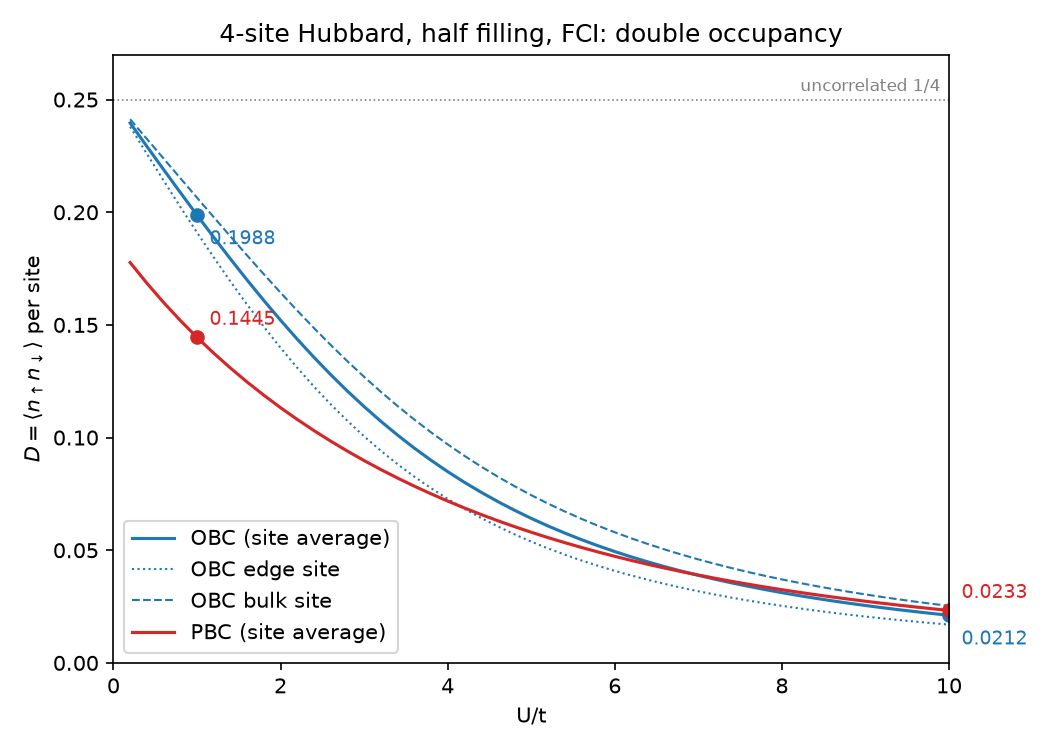
\includegraphics[width=0.62\textwidth]{../hubbard4_fci/plots/docc_vs_U.png}
  \caption{FCI double occupancy per site vs.\ $U/t$ (the $U=0$ point is left out). Script
  \texttt{plot\_hubbard4\_docc.py}.}
  \label{fig:fci_docc}
\end{figure}

\begin{figure}[H]
  \centering
  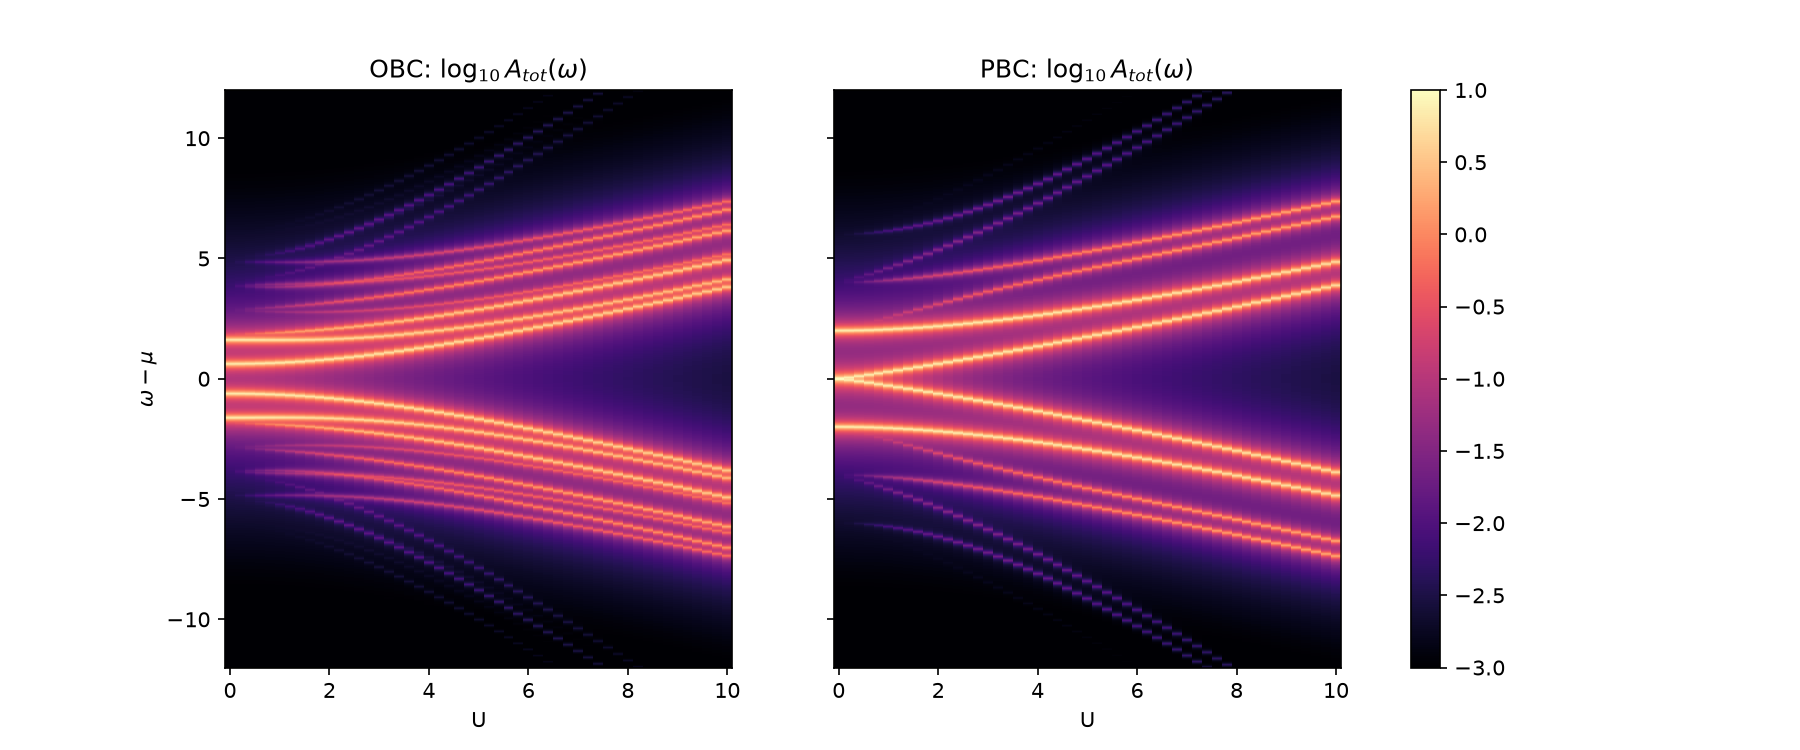
\includegraphics[width=\textwidth]{../hubbard4_fci/plots/A_tot_vs_U.png}
  \caption{FCI total spectral function $\log_{10}A_{tot}(\omega)$ vs.\ $U/t$. Script
  \texttt{plot\_hubbard4\_fci.py}.}
  \label{fig:fci_map}
\end{figure}

\paragraph{Analysis.}
Everything is smooth in $U$: the gap opens continuously (from $0$ for PBC, from the finite-size gap
for OBC and APBC) and grows as $U-\mathrm{const}$ once $U\gtrsim4t$ (the bandwidth); the spectral weight moves
into lower and upper Hubbard bands, each with internal structure; $D$ decays as $\sim c\,t^2/U^2$ and never
reaches zero. A finite cluster cannot have a phase transition, and the half-filled 1D Hubbard model
is insulating for every $U>0$ anyway: what the FCI shows is a band-to-Mott crossover around $U\approx3$--$4t$.

%=====================================================================
\section{Gutzwiller results}
\label{sec:gutz}

\paragraph{Setup.} Four single-site fragments, $\Ng=0$ (ordinary Gutzwiller), $\Ng=2$ and $\Ng=4$ ghosts per site,
paramagnetic, $N_\uparrow=N_\downarrow=2$ fixed. For each geometry and $\Ng$
(\texttt{scripts/scan\_4site\_cpp.py}):
\begin{itemize}[nosep]
  \item \emph{forward} sweep $U=0\to20$, \emph{backward} sweep $U=20\to0$, each point seeded with the previous point's
        converged $(R,\lambda)$. $\Ng=0$: forward starts from $R=1,\lambda=0$, backward from the forward $U=20$ solution.
        $\Ng=2$: a cold start lands on the sleeping-ghost branch, so the forward sweep starts from the dimer solution
        \texttt{examples/U2\_backward} and the backward one from \texttt{examples/U10} (dimer atom 0 $\to$ sites 1,3;
        atom 1 $\to$ sites 2,4). $\Ng=4$: the same, from the converged $\Ng=4$ dimer solutions at $U=2$ and $U=10$
        (\texttt{scan\_ng4\_not\_imp/U\_\{2,10\}.0}, copied to \texttt{scan\_4site\_ng4/seeds/});
  \item \emph{polish} (\texttt{scripts/polish\_4site\_cpp.py}): alternating up/down re-sweeps, each $U$ reseeded from the
        current best solution at the neighbouring $U$, until nothing improves.
\end{itemize}
Only the lowest converged energy per $U$ is shown. Convergence: $|\Delta E|,|\Delta\mathrm{mat}|<10^{-8}$; the code prints
$\Evar$ to $\sim6$ significant digits. The $|R|^2$ shown is the norm of the 1$\times$(1+$\Ng$) row $R_i$ (for $\Ng>0$ it is not the
quasiparticle weight).

\paragraph{PBC caveat.} With PBC the quasiparticle Hamiltonian has the same degenerate pair at the Fermi level as
at $U=0$, and the code fills it with an integer occupation. The solution becomes a charge-density wave
(densities per spin $0.29/0.71$ on alternating sites at $U=1$), $D$ exceeds $0.25$, and the energy can lie above the
$R=0$ insulator. PBC Gutzwiller results are therefore unreliable; APBC is the closed-shell ring to use.

\subsection{$\Ng=0$ (ordinary Gutzwiller)}

\begin{figure}[H]
  \centering
  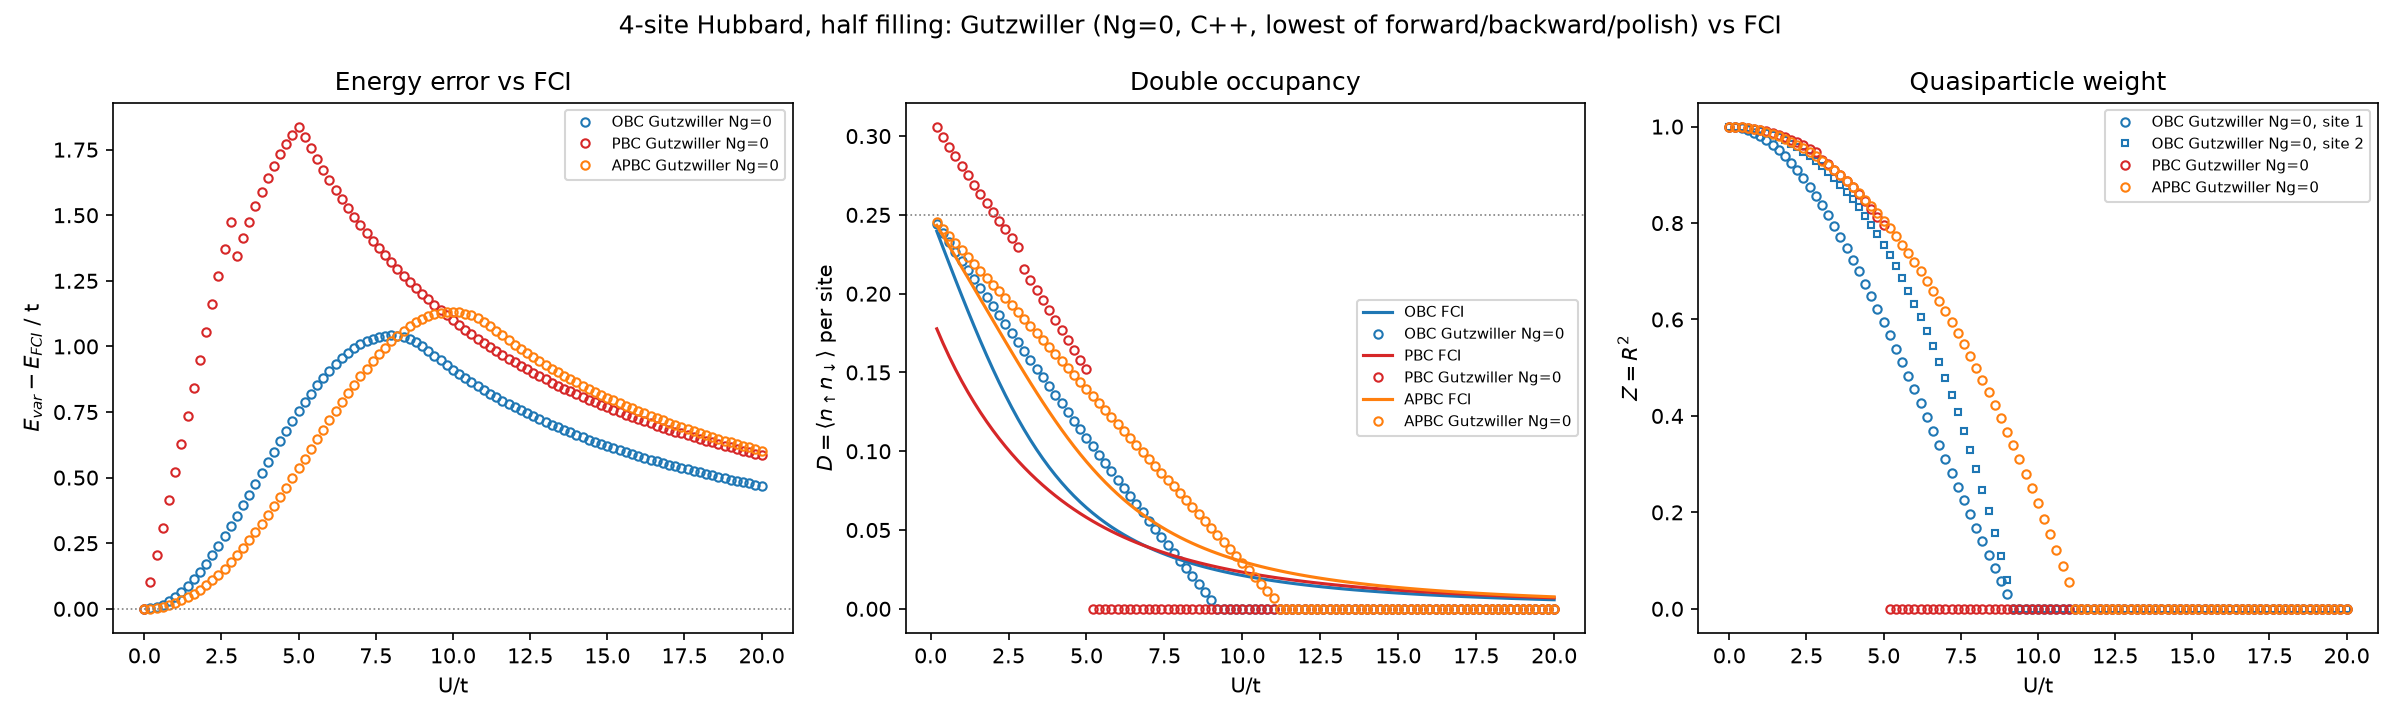
\includegraphics[width=\textwidth]{../scan_4site_ng0/gutz_vs_fci.png}
  \caption{$\Ng=0$: energy error $\Evar-\EFCI$, double occupancy and $|R|^2$ vs.\ $U/t$ (lowest branch). Script
  \texttt{plot\_4site\_gutz\_vs\_fci.py}.}
  \label{fig:ng0}
\end{figure}

A Brinkman--Rice transition: $R\to0$ at $U_c/t$ between $9.0$ and $9.2$ (OBC) and between $11.0$ and $11.2$ (APBC), and
$D$ falls almost linearly to zero there. The edge sites of the chain lose weight first. Above $U_c$ the solution
is the atomic insulator, $R=0$, $\Evar=-2U$ exactly, $D=0$, so the error equals the FCI kinetic (superexchange) energy.
The error peaks just below $U_c$: $1.04$ at $U=8$ (OBC), $1.13$ at $U=10$ (APBC).
The $R=0$ state is a fixed point of the iteration below $U_c$ too (the backward sweep stays on it), but it is higher in energy there.

\subsection{$\Ng=2$}

\begin{figure}[H]
  \centering
  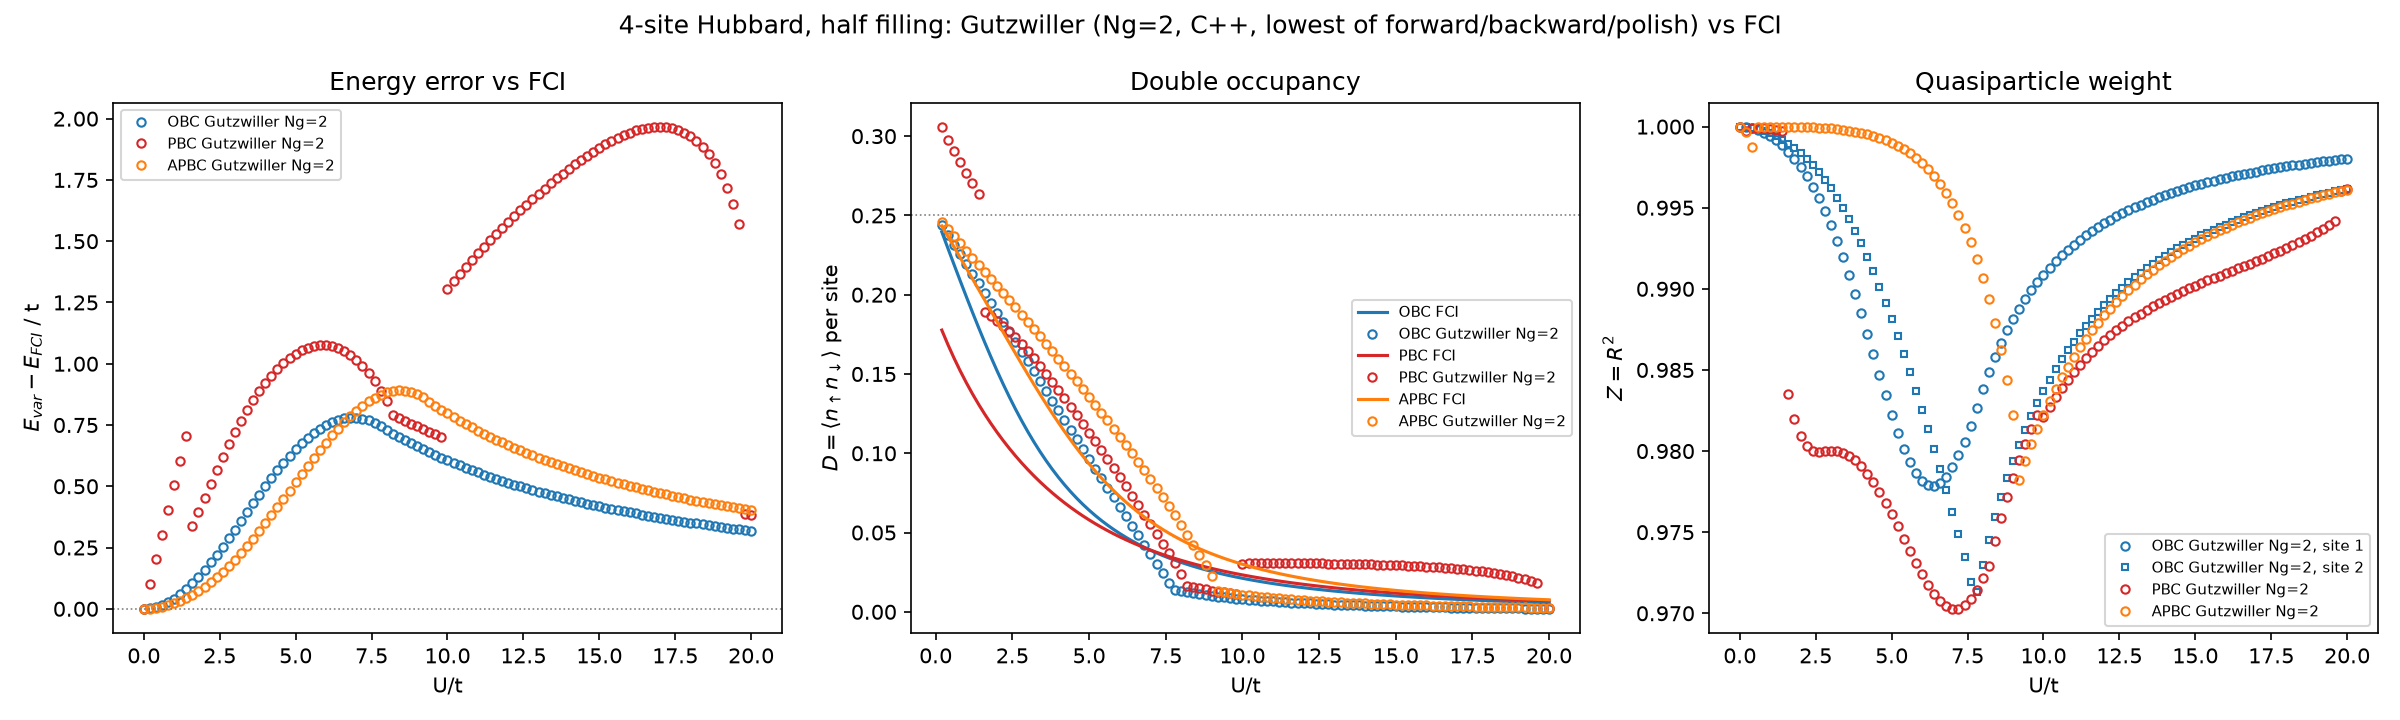
\includegraphics[width=\textwidth]{../scan_4site_ng2/gutz_vs_fci.png}
  \caption{$\Ng=2$: as Fig.~\ref{fig:ng0}.}
  \label{fig:ng2}
\end{figure}

With ghosts there is no transition: $|R|^2$ stays $\gtrsim0.97$, $D$ stays finite and is close to FCI at large
$U$, and the error is bounded (maximum $0.78$ at $U=6.8$ for OBC, $0.89$ at $U=8.4$ for APBC) and decays at
large $U$. At small $U$ the best $\Ng=2$ solution is hardly better than $\Ng=0$ (for APBC up to $U\approx6$ it is the
sleeping-ghost solution, identical to $\Ng=0$); above $U\approx7$ the ghost-active branch wins.
The polish step lowered 16 APBC points ($U=6$--$9$, by up to $0.12t$) and removed a branch jump there.

\subsection{$\Ng=4$}

\begin{figure}[H]
  \centering
  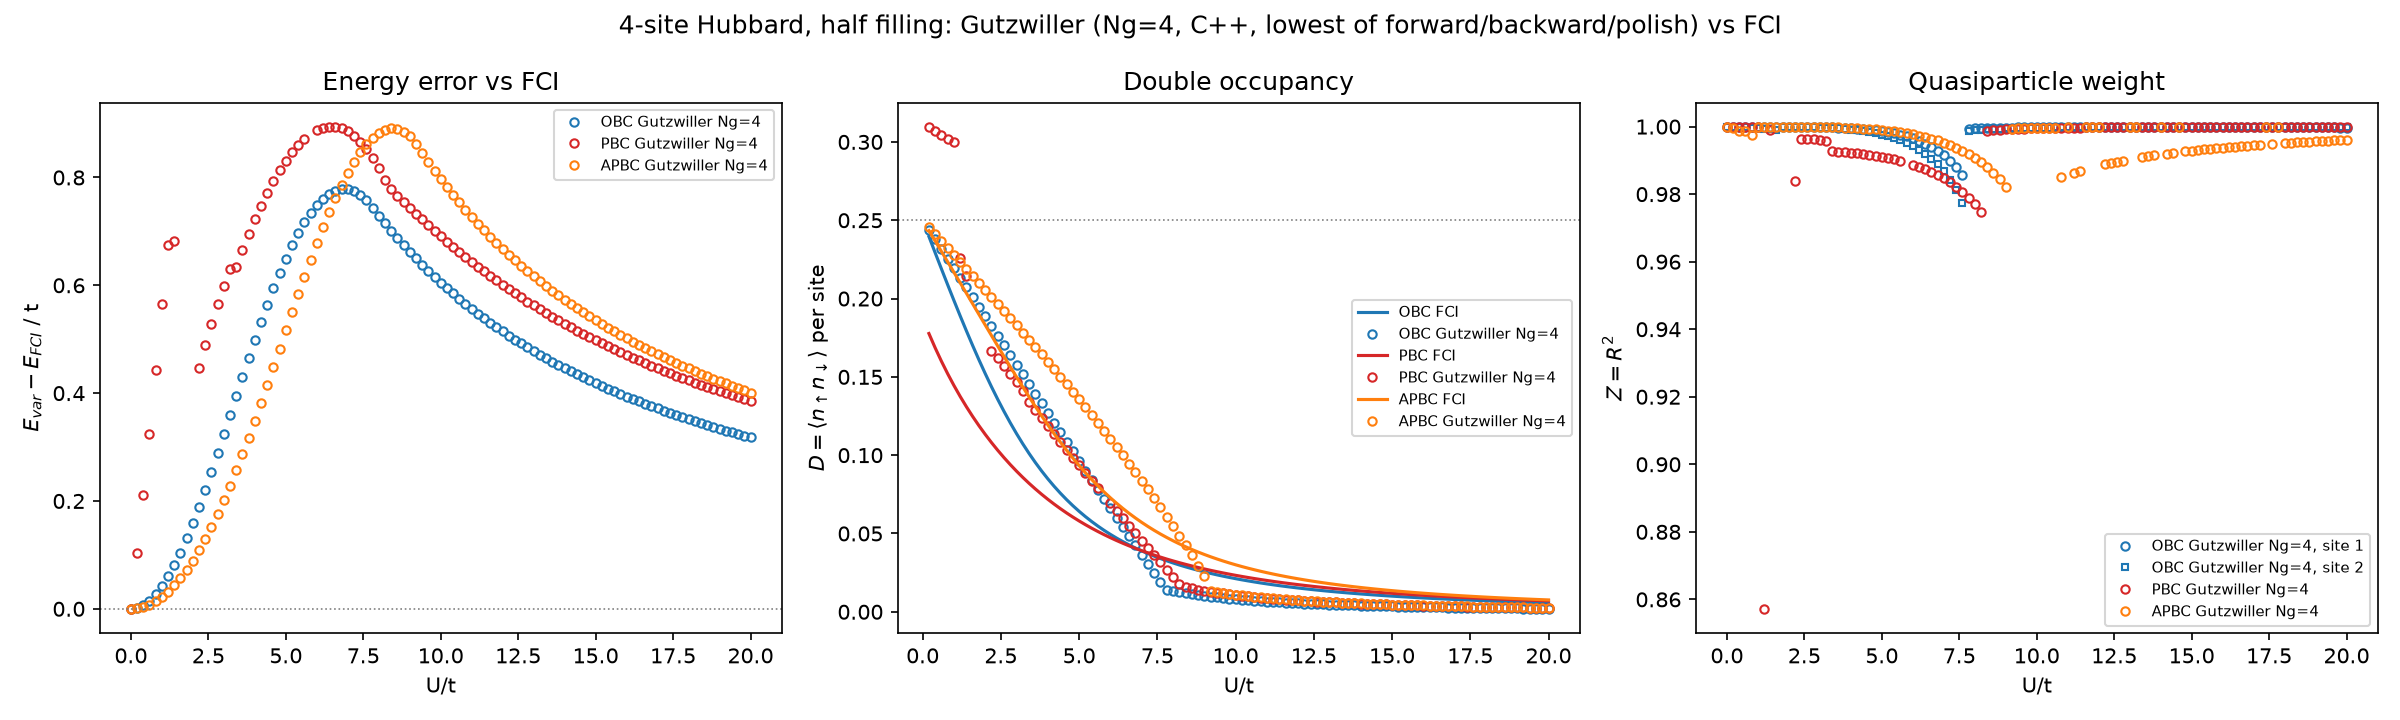
\includegraphics[width=\textwidth]{../scan_4site_ng4/gutz_vs_fci.png}
  \caption{$\Ng=4$: as Fig.~\ref{fig:ng0}. PBC has no converged solution at $U=1.6$, $1.8$, $2.0$ and $5.8$.}
  \label{fig:ng4}
\end{figure}

For OBC and APBC, $\Ng=4$ gives the same energies as $\Ng=2$ to within $10^{-3}t$ (largest gain $9\times10^{-4}$ for OBC near
$U=5$, otherwise $\lesssim10^{-4}$): same maximum error ($0.78$ at $U=6.8$, OBC; $0.89$ at $U=8.4$, APBC), same $D$, $|R|^2\geq0.98$.
Forward and backward sweeps end on the same solution, all 101 points converge, and polishing changed only 4 APBC
points ($U=1$--$1.6$, by $\leq5\times10^{-5}$), so the $\Ng=4$ curves have no branch jumps. With one-site fragments,
going from two to four ghosts per site therefore does not improve the energy: either $\Ng=2$ already saturates
this ansatz or the extra ghosts are redundant (not checked).
For PBC, $\Ng=4$ is smoother than $\Ng=2$: the jumps at $U\approx10$--$15$ are gone and above $U\approx6$ the error is close
to APBC ($0.69$ at $U=10$ vs.\ $1.31$ for $\Ng=2$). At small $U$ it still has the CDW artifact ($D\approx0.30>0.25$).
Convergence for PBC is slow ($\sim2$ min per point vs.\ $\sim9$ s for OBC/APBC).

\begin{table}[H]
\centering
\caption{Energy error $\Evar-\EFCI$ ($t=1$) of the lowest Gutzwiller solution.}
\label{tab:err}
\begin{tabular}{r rrr rrr}
\toprule
 & \multicolumn{3}{c}{OBC} & \multicolumn{3}{c}{APBC}\\
\cmidrule(lr){2-4}\cmidrule(lr){5-7}
$U/t$ & $\Ng=0$ & $\Ng=2$ & $\Ng=4$ & $\Ng=0$ & $\Ng=2$ & $\Ng=4$\\
\midrule
 1 & 0.045 & 0.042 & 0.042 & 0.022 & 0.022 & 0.022\\
 2 & 0.172 & 0.159 & 0.159 & 0.090 & 0.089 & 0.089\\
 4 & 0.559 & 0.499 & 0.499 & 0.357 & 0.349 & 0.349\\
 6 & 0.908 & 0.750 & 0.749 & 0.719 & 0.678 & 0.678\\
 8 & 1.042 & 0.730 & 0.729 & 1.019 & 0.883 & 0.883\\
10 & 0.912 & 0.605 & 0.605 & 1.132 & 0.798 & 0.797\\
15 & 0.620 & 0.418 & 0.418 & 0.805 & 0.535 & 0.535\\
20 & 0.469 & 0.318 & 0.318 & 0.603 & 0.401 & 0.401\\
\bottomrule
\end{tabular}
\end{table}

%=====================================================================
\section{Spectral functions}
\label{sec:spectra}

The Gutzwiller Green's function is the one evaluated by \texttt{run\_ggut} on the same grid as FCI
($\omega\in[-20,20]$, 8001 points, $\eta=0.05$, per spin, all $4\times4$ elements).

\begin{figure}[H]
  \centering
  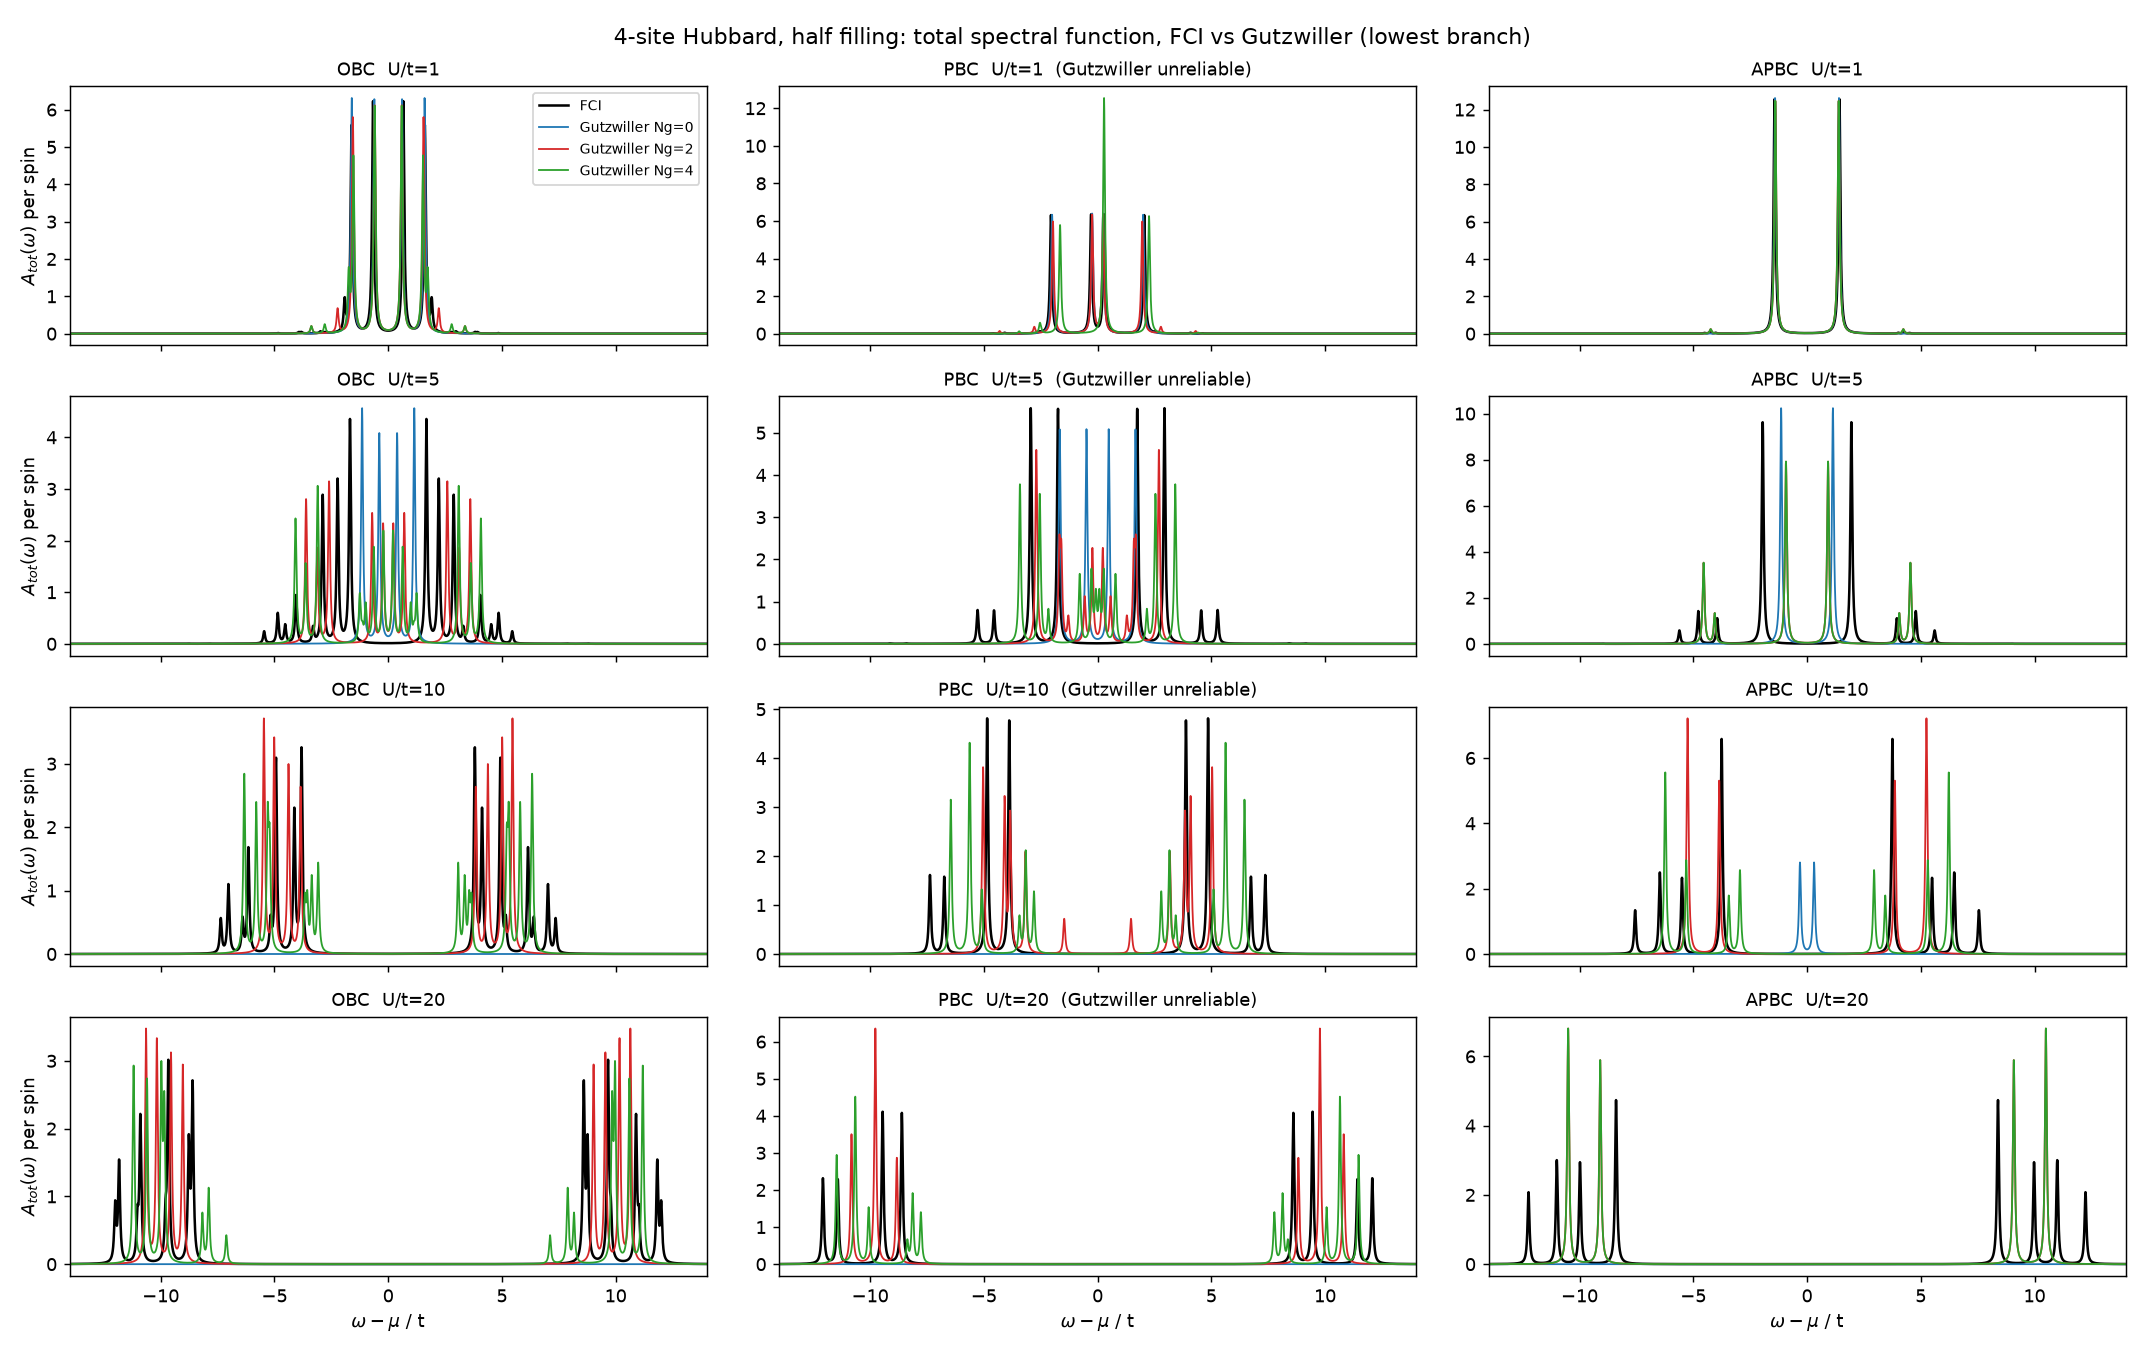
\includegraphics[width=\textwidth]{../hubbard4_fci/plots/spectra_gutz_vs_fci.png}
  \caption{Total spectral function $A_{tot}=\sum_iA_{ii}$: FCI (black), Gutzwiller $\Ng=0$ (blue), $\Ng=2$ (red) and $\Ng=4$ (green),
  lowest branch, at $U/t=1,5,10,20$. Script \texttt{plot\_4site\_spectra\_gutz\_vs\_fci.py}.}
  \label{fig:spec}
\end{figure}

\begin{figure}[H]
  \centering
  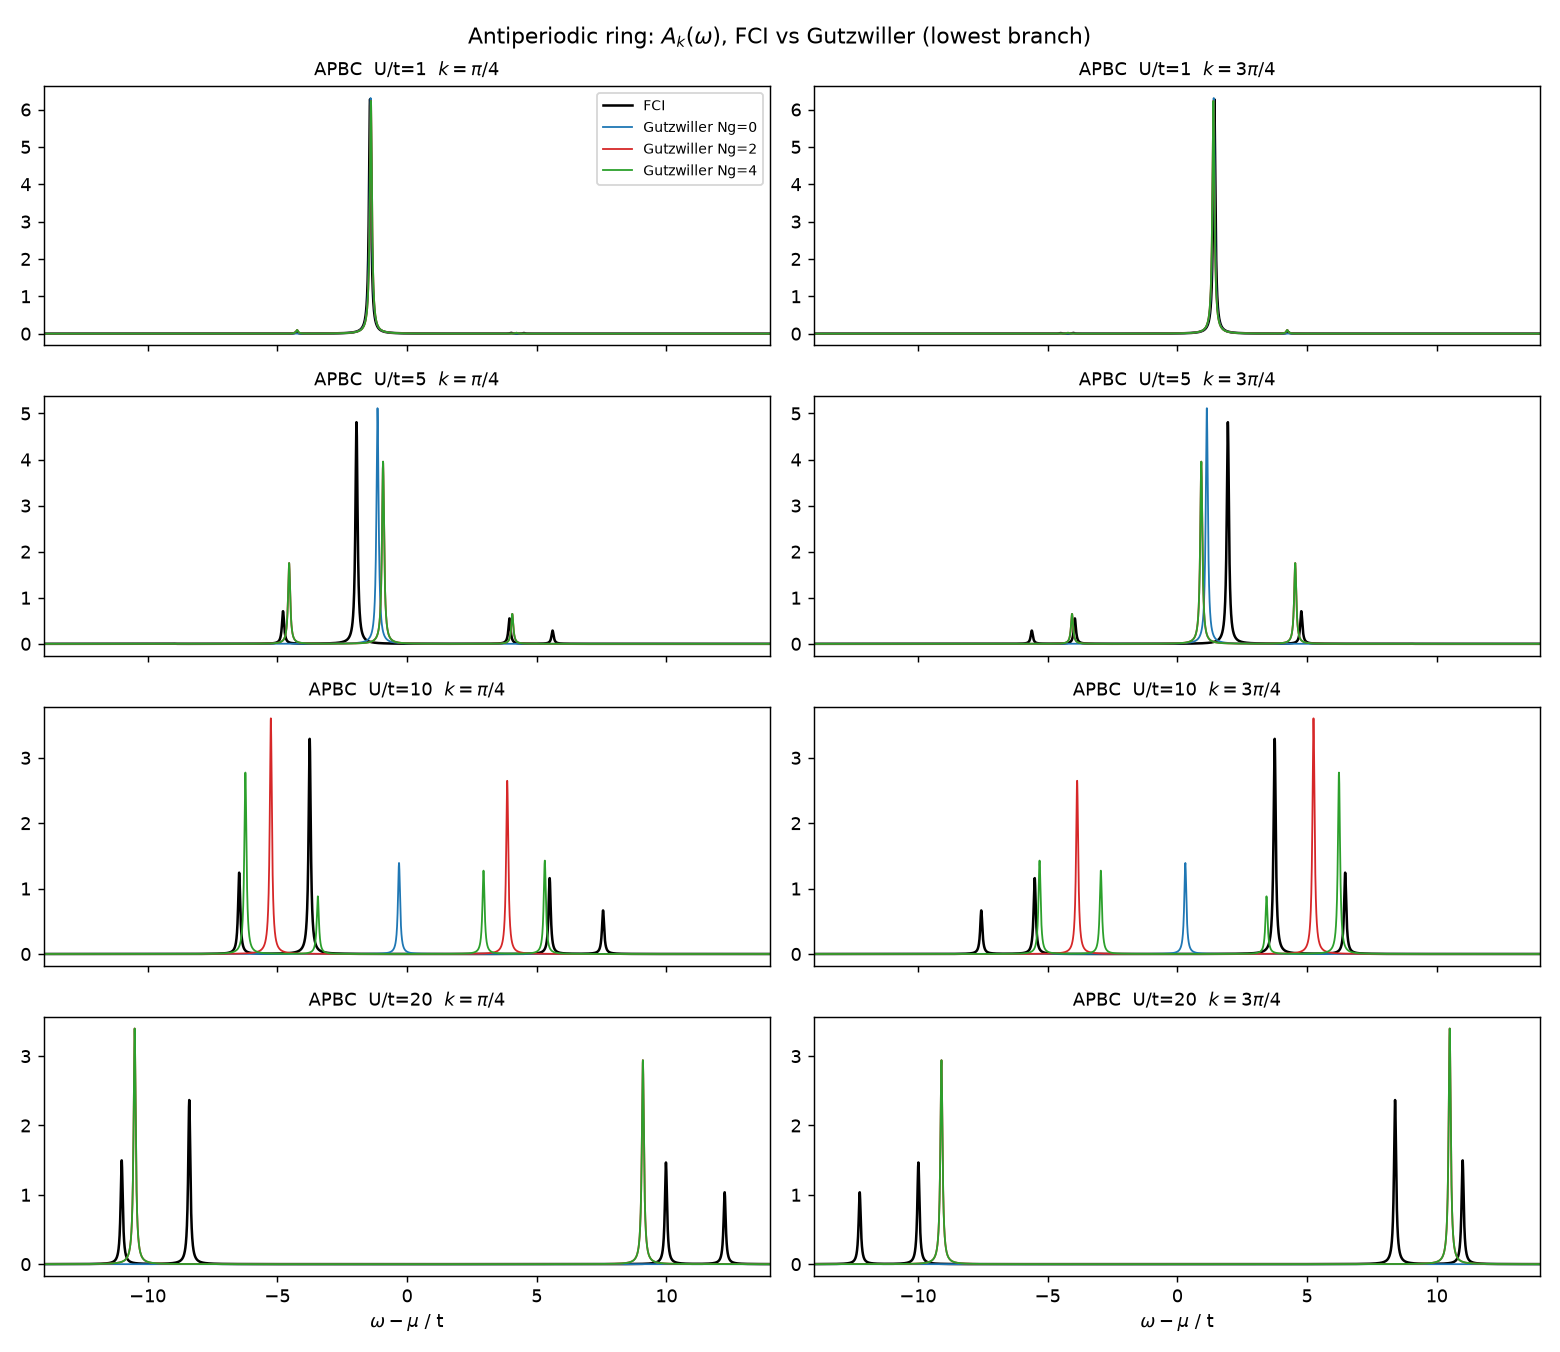
\includegraphics[width=0.9\textwidth]{../hubbard4_fci/plots/spectra_k_gutz_vs_fci_apbc.png}
  \caption{APBC, momentum-resolved $A_k(\omega)$ at $k=\pi/4$ and $3\pi/4$ ($7\pi/4$ and $5\pi/4$ are identical by symmetry).}
  \label{fig:speck}
\end{figure}

\paragraph{Analysis.}
At $U=1$ both $\Ng$ reproduce the FCI peaks (the ghosts also give the small satellites). For $\Ng=0$ only the
renormalized quasiparticle peaks exist: they are pulled towards $\omega=0$ by $Z$, there are no Hubbard bands,
and above $U_c$ the spectral function is zero. With $\Ng=2$ lower and upper Hubbard bands appear with roughly the
right gap (APBC $U=20$: peaks at $\pm9$--$10.5$ vs.\ FCI $\pm8.4$--$12.3$), but each band is 2--3 sharp peaks where FCI
has 3--4 spread over a wider range. In the $k$-resolved APBC spectra the main peaks have about the right weight and
position; the FCI satellites are only partly captured, as single shifted peaks. The worst case is OBC at $U\approx5$,
where $\Ng=2$ puts peaks inside the FCI gap region, the same $U$ range where the energy error peaks.

Although $\Ng=4$ and $\Ng=2$ have the same energies, their spectra are not the same. For APBC they coincide at
$U=1$ and $U=20$ (peaks at $\pm9.1$, $\pm10.5$), but at $U=5$ and $10$ $\Ng=4$ spreads each Hubbard band over more peaks.
For OBC at $U=20$, $\Ng=4$ gives 7 peaks per band ($7.1$--$11.2$, vs.\ $9.0$--$10.6$ for $\Ng=2$), some of them about
$1$--$2t$ closer to the gap than in FCI. Neither $\Ng$ reproduces the FCI peak positions in detail at large $U$, and
equal total energies do not imply equally good spectra.

\subsection{Spectral function movies}

One frame per $U/t$ ($0\to20$, step $0.2$): Gutzwiller $A_{tot}(\omega)$ of the lowest branch (filled) vs.\ FCI (red);
the frame also gives $\Evar-\EFCI$ and $|R_1|^2$ (script \texttt{make\_4site\_A\_omega\_video.py}).
\begin{itemize}[nosep]
  \item $\Ng=0$: \href{run:../scan_4site_ng0/obc/A_omega_vs_U.mp4}{OBC},
        \href{run:../scan_4site_ng0/apbc/A_omega_vs_U.mp4}{APBC},
        \href{run:../scan_4site_ng0/pbc/A_omega_vs_U.mp4}{PBC (unreliable)}
  \item $\Ng=2$: \href{run:../scan_4site_ng2/obc/A_omega_vs_U.mp4}{OBC},
        \href{run:../scan_4site_ng2/apbc/A_omega_vs_U.mp4}{APBC},
        \href{run:../scan_4site_ng2/pbc/A_omega_vs_U.mp4}{PBC (unreliable)}
  \item $\Ng=4$: \href{run:../scan_4site_ng4/obc/A_omega_vs_U.mp4}{OBC},
        \href{run:../scan_4site_ng4/apbc/A_omega_vs_U.mp4}{APBC},
        \href{run:../scan_4site_ng4/pbc/A_omega_vs_U.mp4}{PBC (unreliable)}
\end{itemize}
\noindent (Links open the movie with the PDF viewer's associated application, if the viewer supports \texttt{run:} links.)

%=====================================================================
\section{Summary}
\label{sec:summary}

\begin{itemize}[nosep]
  \item FCI: smooth band-to-Mott crossover around $U\approx3$--$4t$; no transition.
  \item $\Ng=0$: a Brinkman--Rice transition at $U_c\approx9.1t$ (OBC) and $11.1t$ (APBC), an artifact of the method;
        no Hubbard bands; error up to $\sim1.1t$.
  \item $\Ng=2$: no transition, Hubbard bands with about the right gap, error at most $0.78t$ (OBC) and
        $0.89t$ (APBC) and $\sim30\%$ below $\Ng=0$ at large $U$; at small $U$ hardly better than $\Ng=0$.
  \item $\Ng=4$: OBC/APBC energies equal to $\Ng=2$ within $10^{-3}t$, with no branch jumps; the spectra differ
        (more peaks per Hubbard band) but are not closer to FCI. PBC becomes smoother but keeps the small-$U$ CDW artifact.
  \item PBC: the open-shell 4-site ring is not handled by the integer-occupation Gutzwiller code; use APBC.
\end{itemize}

\end{document}
